\chapter{Risultati}
\label{sec:results}

% Source notes: Project/docs/thesis_notes.md (Ch. 6) and checkpoint_2026-10-10.md. Numbers:
% Project/outputs/results/<run>/{t1,t2,t3,calibration,latency,energy}/metrics.json; bootstrap: results/bootstrap/summary.md.
% Figures: Project/outputs/figures/{benchmarks,bootstrap,training-*,calibration-*}/ (copied to Thesis/images/results/).

Questo capitolo illustra come GroundOne apprende e quanto è stabile il suo addestramento, quali risultati ottiene sui tre
test set congelati, come si colloca rispetto alle baseline e quale contributo dia, di per sé, il readout del System One.
Esamina poi la qualità delle probabilità, il tempo e l'energia necessari per verificare una risposta e gli errori che
restano. Gli intervalli sono intervalli di confidenza al 95\,\% ottenuti con un bootstrap a cluster, calcolati come
descritto nella Sezione~\ref{sec:setup-statistics}.

\section{Addestramento}
\label{sec:results-training}

Entrambi i modelli hanno appreso il task. Prima dell'addestramento, un modello che legge il formato con i marker non
sa che cosa il marker gli chieda e i suoi verdetti sono casuali: il 0.5B risponde ``contraddetta'' per l'88\,\% delle
frasi del dev set e raggiunge una balanced accuracy a tre classi di 0.32. Nelle esecuzioni completate la loss di
addestramento è scesa, già nei primi cento passi, sotto il valore di un modello che conosca soltanto le frequenze delle
classi ($\ln 3 \approx 1.10$), e il punteggio sul dev set è poi cresciuto con regolarità (Figura~\ref{fig:results-dev}).
Il 0.5B, addestrato su tutte le 13{,}203 risposte, ha toccato il punteggio migliore al passo 600 di 802, con una balanced
accuracy di 0.633 in media sui tre task, per poi stabilizzarsi. Il 3B, addestrato per 12.25 ore su 6{,}500 risposte,
ha raggiunto 0.705 al passo 320 di 403 sul proprio sottoinsieme del dev set. Sull'intero dev set la balanced accuracy a
tre classi è di 0.731 per il 0.5B e di 0.784 per il 3B, e in entrambe le esecuzioni tutte e tre le classi sono rimaste
presenti fra le predizioni per tutto l'addestramento.

\begin{figure}[htbp]
\centering
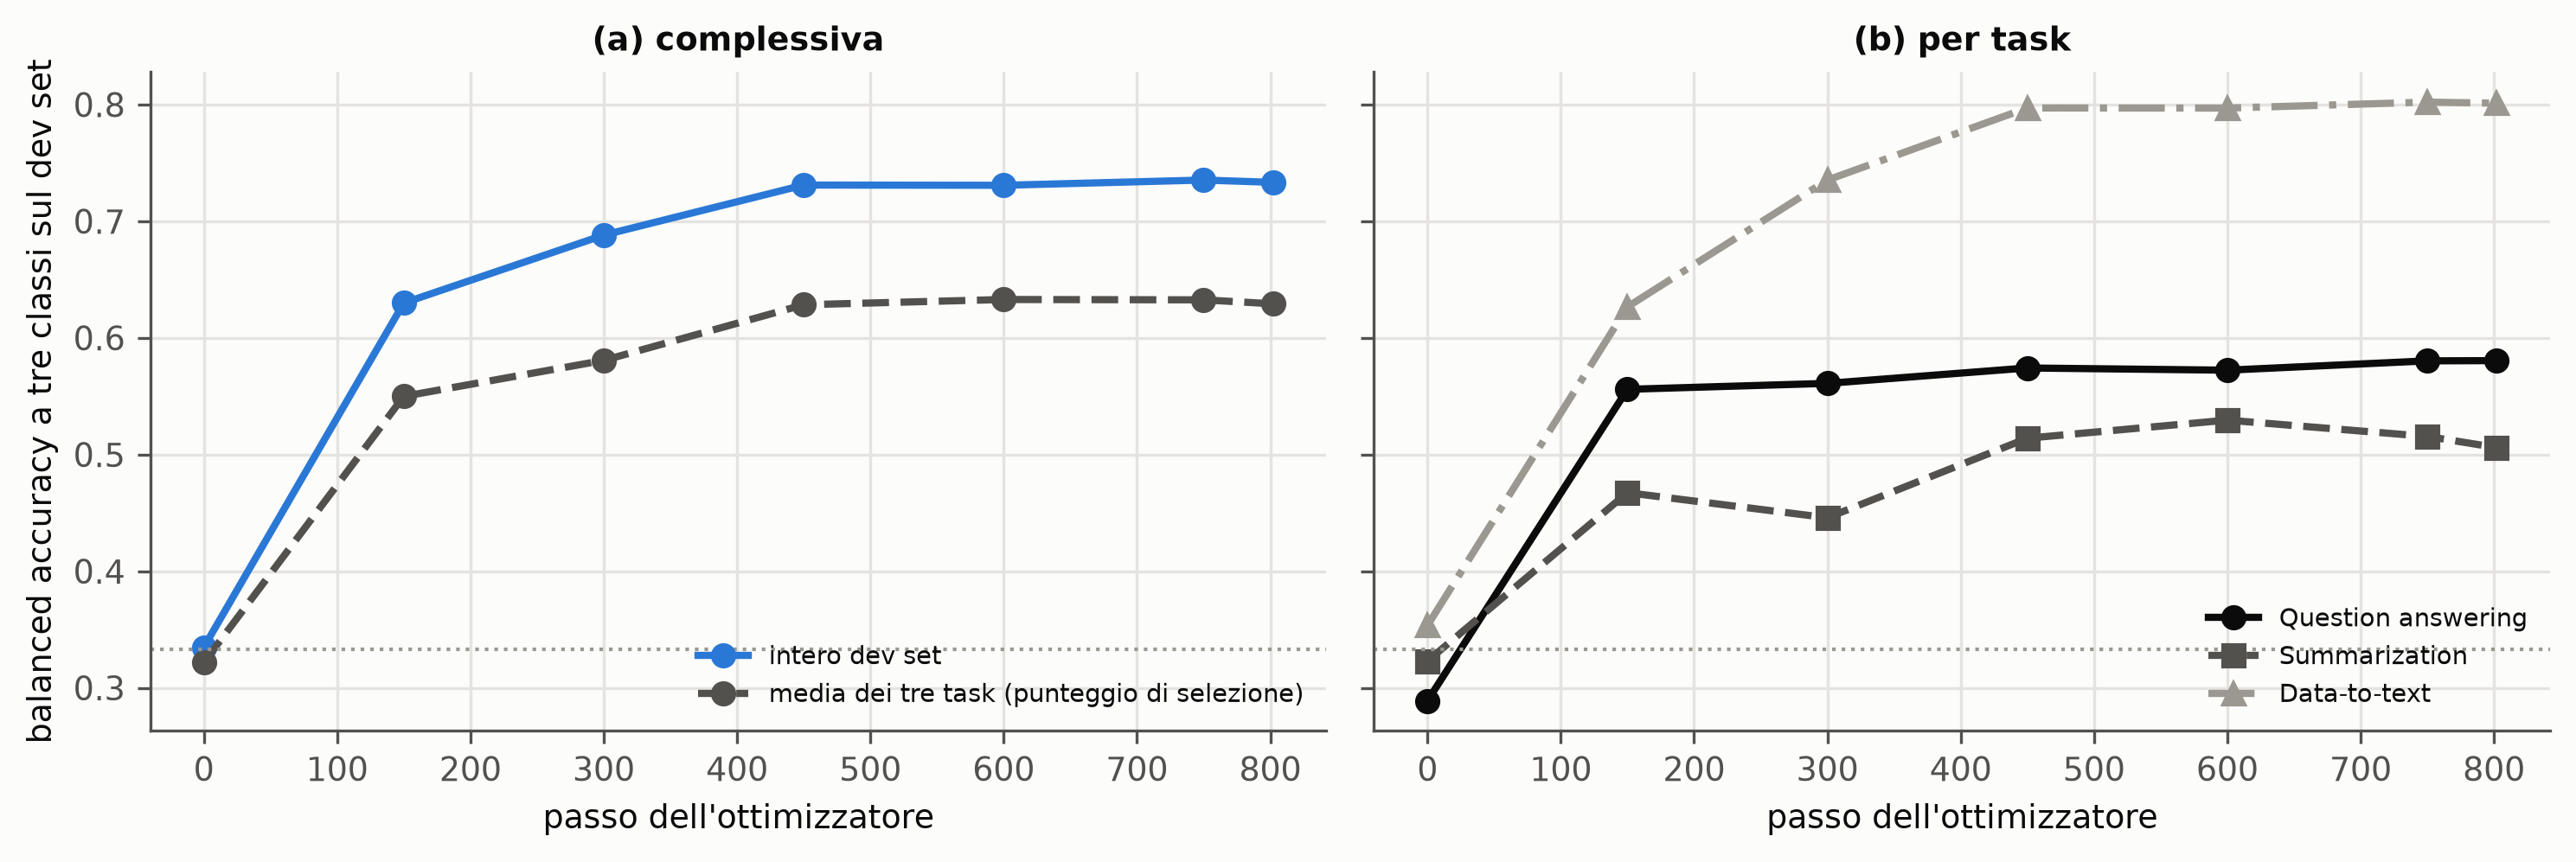
\includegraphics[width=\textwidth]{images/results/g1-05b-dev_bacc.png}
\caption{Balanced accuracy a tre classi sul dev set durante l'addestramento del modello 0.5B, complessiva (a sinistra) e
per task (a destra). La linea punteggiata indica il livello casuale. Il 3B mostra lo stesso andamento sul suo
sottoinsieme di 200 risposte del dev set.}
\label{fig:results-dev}
\end{figure}

\section{Variabilità tra seed}
\label{sec:results-seeds}

La procedura del 0.5B è stata ripetuta con un secondo seed, che cambia l'inizializzazione degli adapter e l'ordine dei
batch. Quando l'addestramento converge, converge allo stesso punto (Figura~\ref{fig:results-seeds}): la seconda
esecuzione raggiunge su T1 una balanced accuracy a tre classi di 0.767 contro 0.769 e un AUROC di 0.907 contro 0.905,
su LLM-AggreFact 71.5 contro 70.1 e su VitaminC 0.434 contro 0.442. Su T1 la differenza appaiata è $+0.001$ (da $-0.008$
a $+0.011$) e non è significativa. Le differenze emergono nei dettagli. Gli errori si distribuiscono in modo diverso tra
le classi, con la recall delle frasi supportate e di quelle non menzionate che si sposta di circa 0.04 in direzioni
opposte, e le porzioni più piccole dei dati oscillano di più: di 0.023 la fascia con quattordici o più decisioni, di
0.025 l'AUROC su VitaminC e fino a dieci punti i singoli dataset di LLM-AggreFact, come WiCE (67.9 contro 78.0).

\begin{figure}[htbp]
\centering
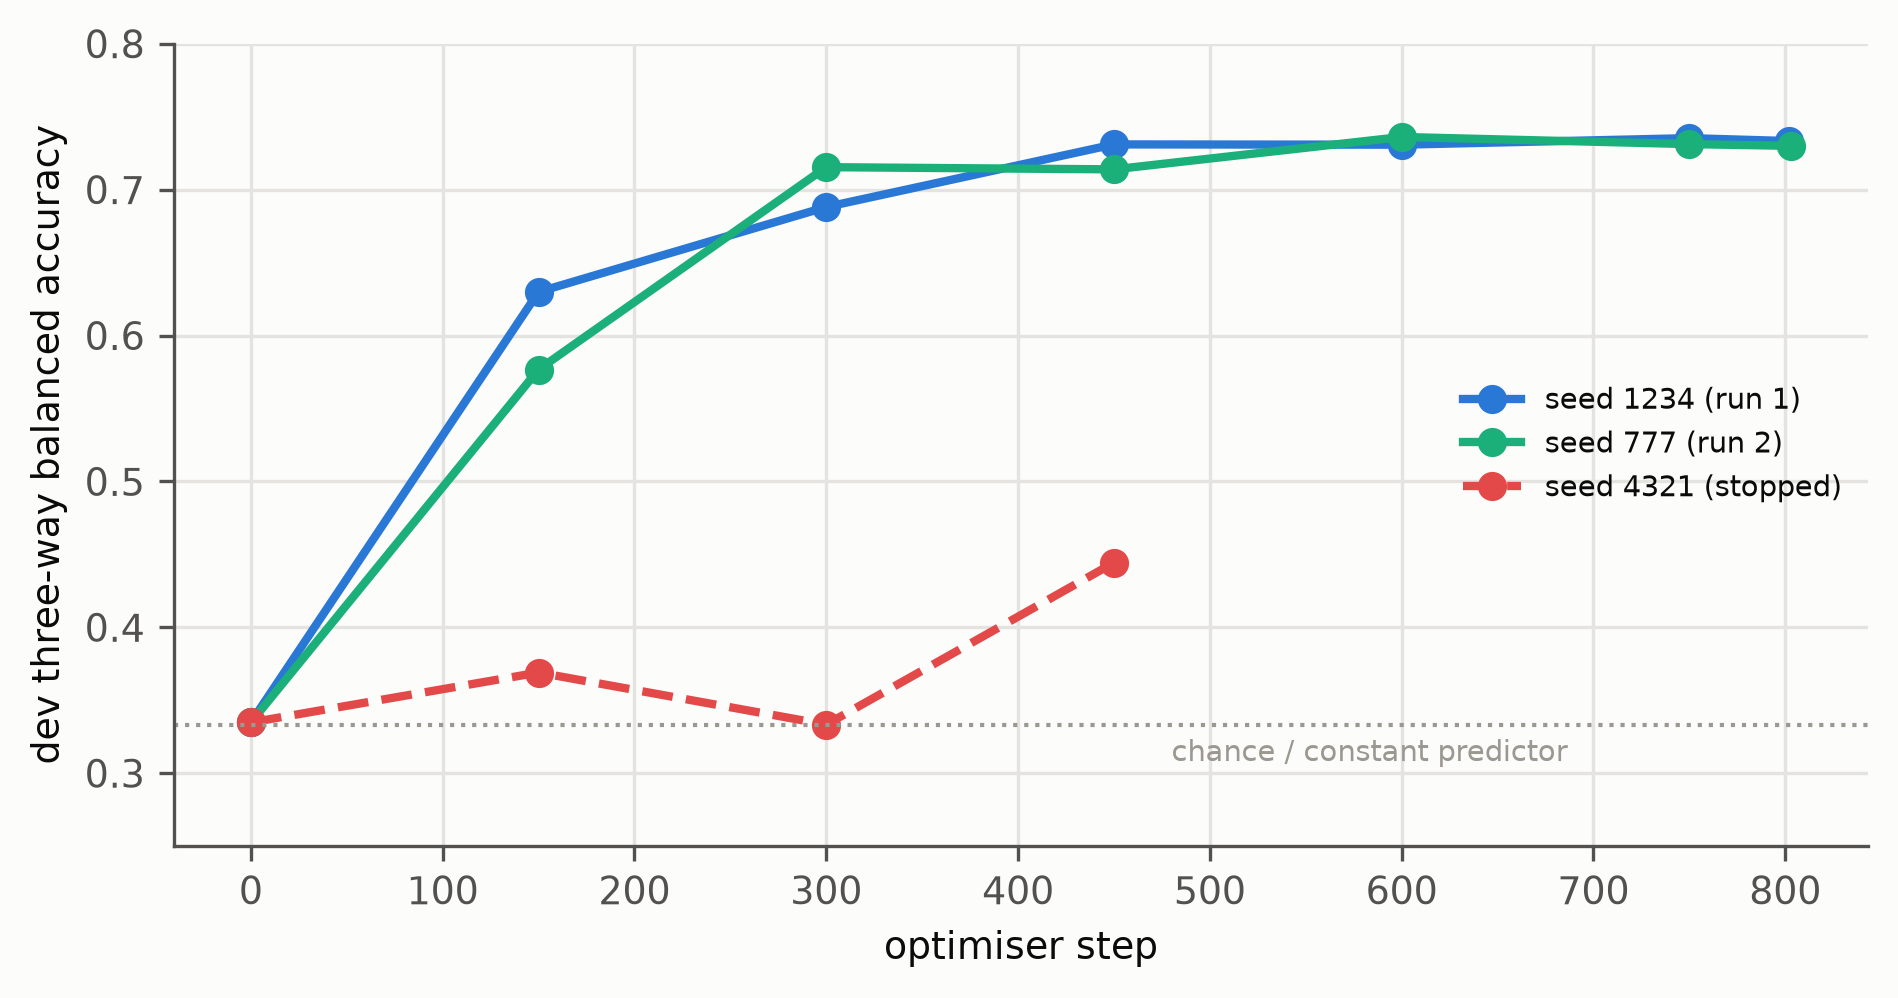
\includegraphics[width=0.85\textwidth]{images/results/seed_runs_05b.png}
\caption{Balanced accuracy a tre classi sul dev set del modello 0.5B durante l'addestramento, con la stessa procedura e
tre seed. Due esecuzioni convergono allo stesso livello; la terza è collassata su un predittore costante ed è stata
interrotta.}
\label{fig:results-seeds}
\end{figure}

Ne seguono due conseguenze. La prima è che il bootstrap, che ricampiona i dati di test, non coglie questa fonte di
variabilità: su LLM-AggreFact e su VitaminC le due esecuzioni della stessa procedura differiscono più di quanto i loro
intervalli consentirebbero ($-0.013$ sulla media macro di T2, $-0.025$ sull'AUROC di T3). Le differenze tra sistemi
inferiori alla dispersione tra seed, cioè circa 1.5 punti sulla media macro di LLM-AggreFact e 0.025 di AUROC su
VitaminC, non vengono pertanto interpretate, e lo stesso vale per i singoli dataset di LLM-AggreFact quando lo scarto non
supera circa cinque punti.

La seconda è che l'addestramento non sempre converge. Un'esecuzione con un terzo seed è rimasta vicina al livello
casuale: il suo punteggio sul dev set era 0.369 al passo 150 e 0.333 al passo 300, quando prediceva ``supportata'' per
ogni frase, e la loss di addestramento è rimasta prossima a quella di un modello privo di informazione. L'esecuzione è
stata interrotta al passo 470 di 801, quando il punteggio era risalito a 0.444; non è quindi possibile sapere se si
sarebbe ripresa entro la fine dell'epoca, e in quanto incompleta è esclusa dalle tabelle. La procedura ha due
caratteristiche note per rendere fragile il fine-tuning: non applica gradient clipping e l'ottimizzatore lavora senza
bias correction, l'impostazione predefinita del framework, che è stata indicata come una delle cause principali dei
fine-tuning non riusciti~\cite{pascanu2013difficulty,mosbach2021stability}. Un solo collasso su tre esecuzioni non
basta a stimare un tasso di fallimento, ma mostra che la procedura non è del tutto robusta rispetto
all'inizializzazione.

\section{Accuratezza sul test set RAG (T1)}
\label{sec:results-t1}

Sulle 17{,}284 frasi di T1 il modello 0.5B raggiunge una balanced accuracy a tre classi di 0.769 e il 3B di 0.832
(Tabella~\ref{tab:results-t1}); la differenza, $+0.063$ (da $+0.052$ a $+0.076$), è l'effetto più netto della
dimensione del modello. Sulla decisione binaria il 0.5B ottiene una balanced accuracy di 0.815 e un AUROC di 0.905, il
3B rispettivamente 0.874 e 0.940. Entrambi superano di gran lunga i segnali che non confrontano mai una frase con il suo
documento: la sovrapposizione lessicale arriva a un AUROC di 0.737 e il classificatore che vede la sola frase a una
balanced accuracy a tre classi di 0.570.

\begin{table}[htbp]
\centering
\caption{GroundOne su T1, per task e per numero di decisioni per risposta ($K$): balanced accuracy a tre classi,
recall delle frasi contraddette e AUROC di $P(\text{supported})$.}
\label{tab:results-t1}
\small
\begin{adjustbox}{max width=\textwidth}
\begin{tabular}{@{}lrrrrrrr@{}}
\toprule
 & & \multicolumn{3}{c}{GroundOne 0.5B} & \multicolumn{3}{c}{GroundOne 3B} \\
\cmidrule(lr){3-5}\cmidrule(l){6-8}
Sottoinsieme & Frasi & Bal.\ acc. & Contr. & AUROC & Bal.\ acc. & Contr. & AUROC \\
\midrule
Tutte & 17{,}284 & 0.769 & 0.68 & 0.905 & 0.832 & 0.76 & 0.940 \\
\midrule
Question answering & 4{,}876 & 0.589 & 0.03 & 0.916 & 0.699 & 0.30 & 0.948 \\
Summarization & 4{,}538 & 0.544 & 0.13 & 0.775 & 0.629 & 0.30 & 0.873 \\
Data-to-text & 7{,}870 & 0.812 & 0.84 & 0.929 & 0.873 & 0.90 & 0.955 \\
\midrule
$K$ = 1--4 & 2{,}434 & 0.606 & 0.18 & 0.857 & 0.677 & 0.25 & 0.921 \\
$K$ = 5--8 & 8{,}012 & 0.758 & 0.67 & 0.899 & 0.829 & 0.78 & 0.936 \\
$K$ = 9--13 & 5{,}201 & 0.824 & 0.82 & 0.926 & 0.863 & 0.86 & 0.945 \\
$K \geq 14$ & 1{,}637 & 0.723 & 0.50 & 0.908 & 0.839 & 0.68 & 0.957 \\
\bottomrule
\end{tabular}
\end{adjustbox}
\end{table}

Spiccano tre aspetti. Il primo è che l'accuratezza non peggiora con la lunghezza della risposta: le risposte con
quattordici o più decisioni sono tra quelle gestite meglio, con 0.723 per il 0.5B e 0.839 per il 3B, mentre la fascia
più difficile è quella delle risposte più brevi, che comprende soprattutto risposte di question answering e di
summarization. Il dato è importante perché è proprio sulle risposte lunghe che un System One fa risparmiare più tempo;
su di esse il guadagno del 3B rispetto al 0.5B è di $+0.116$ (da $+0.050$ a $+0.180$). Il secondo è che le
contraddizioni vengono riconosciute soprattutto nel data-to-text, dove RAGTruth le concentra. Nel question answering e
nella summarization il 0.5B distingue bene le frasi supportate da quelle non menzionate, ma non individua quasi nessuna
contraddizione, con una recall di 0.03 e 0.13. Il 3B porta entrambe a 0.30: la dimensione del modello compensa in parte
la scarsità di questi esempi nei dati di addestramento. Il terzo è che question answering e summarization offrono la
prova più chiara che i modelli leggono davvero il documento: qui il classificatore che vede la sola frase resta al
livello casuale (0.36 e 0.35), mentre i due modelli raggiungono 0.59--0.70 e 0.54--0.63.

Le stesse predizioni si possono leggere anche a livello di risposta intera, che è il criterio con cui il Decision Index
della comunità valuta i decision model generalisti su RAGTruth: una risposta è allucinata se contiene un qualsiasi
contenuto non supportato, e la metrica è l'F1 di questa classe, che un sistema che risponda sempre ``allucinata''
raggiunge già con 0.52~\cite{decisionindex2026}. Prendendo il minimo della $P(\text{supported})$ calibrata sulle frasi
di una risposta, con una soglia stimata sul dev set, GroundOne raggiunge 0.733 con il 0.5B e 0.784 con il 3B sulle
2{,}647 risposte di T1. Nella leaderboard nessun decision model generalista sotto il miliardo di parametri supera 0.55,
Jev raggiunge 0.765 e il modello migliore, da 27B parametri, 0.803. Il confronto è solo indicativo, perché GroundOne è
stato addestrato su RAGTruth, mentre i modelli della leaderboard sono valutati zero-shot, con un prompt diverso e su 53
risposte in più; colloca comunque uno specialista da 0.5B molto al di sopra dei decision model generalisti della stessa
dimensione.

\section{Confronto con le baseline}
\label{sec:results-baselines}

La Figura~\ref{fig:results-comparison} mette a confronto tutti i sistemi su T1. Gli encoder specializzati raggiungono un
AUROC di 0.814 (MiniCheck-RoBERTa) e 0.821 (HHEM), superiore a quello della sovrapposizione lessicale ma inferiore a
quello di entrambi i modelli GroundOne: il 0.5B li supera di $+0.091$ (da $+0.074$ a $+0.107$) e $+0.083$ (da $+0.066$ a
$+0.099$), il 3B di $+0.126$ e $+0.119$. Il confronto per task ridimensiona però questo risultato. Il vantaggio di
GroundOne viene in gran parte dal data-to-text, dove è addestrato nel dominio e dove gli encoder sono più deboli (AUROC
0.71--0.75), mentre nella summarization MiniCheck-RoBERTa supera il modello 0.5B (0.872 contro 0.775) ed è alla pari con
il 3B (0.873). I modelli non addestrati mostrano quanta parte dell'accuratezza si debba all'addestramento: il 0.5B è al
livello casuale perché non risponde mai ``supportata'', e il 3B, a cui si pone la stessa domanda, raggiunge 0.437 contro
0.818 dopo l'addestramento, sulle stesse risposte. Il contributo del readout ristretto, al di là dell'addestramento, è
misurato separatamente nella Sezione~\ref{sec:results-readout}.

\begin{figure}[htbp]
\centering
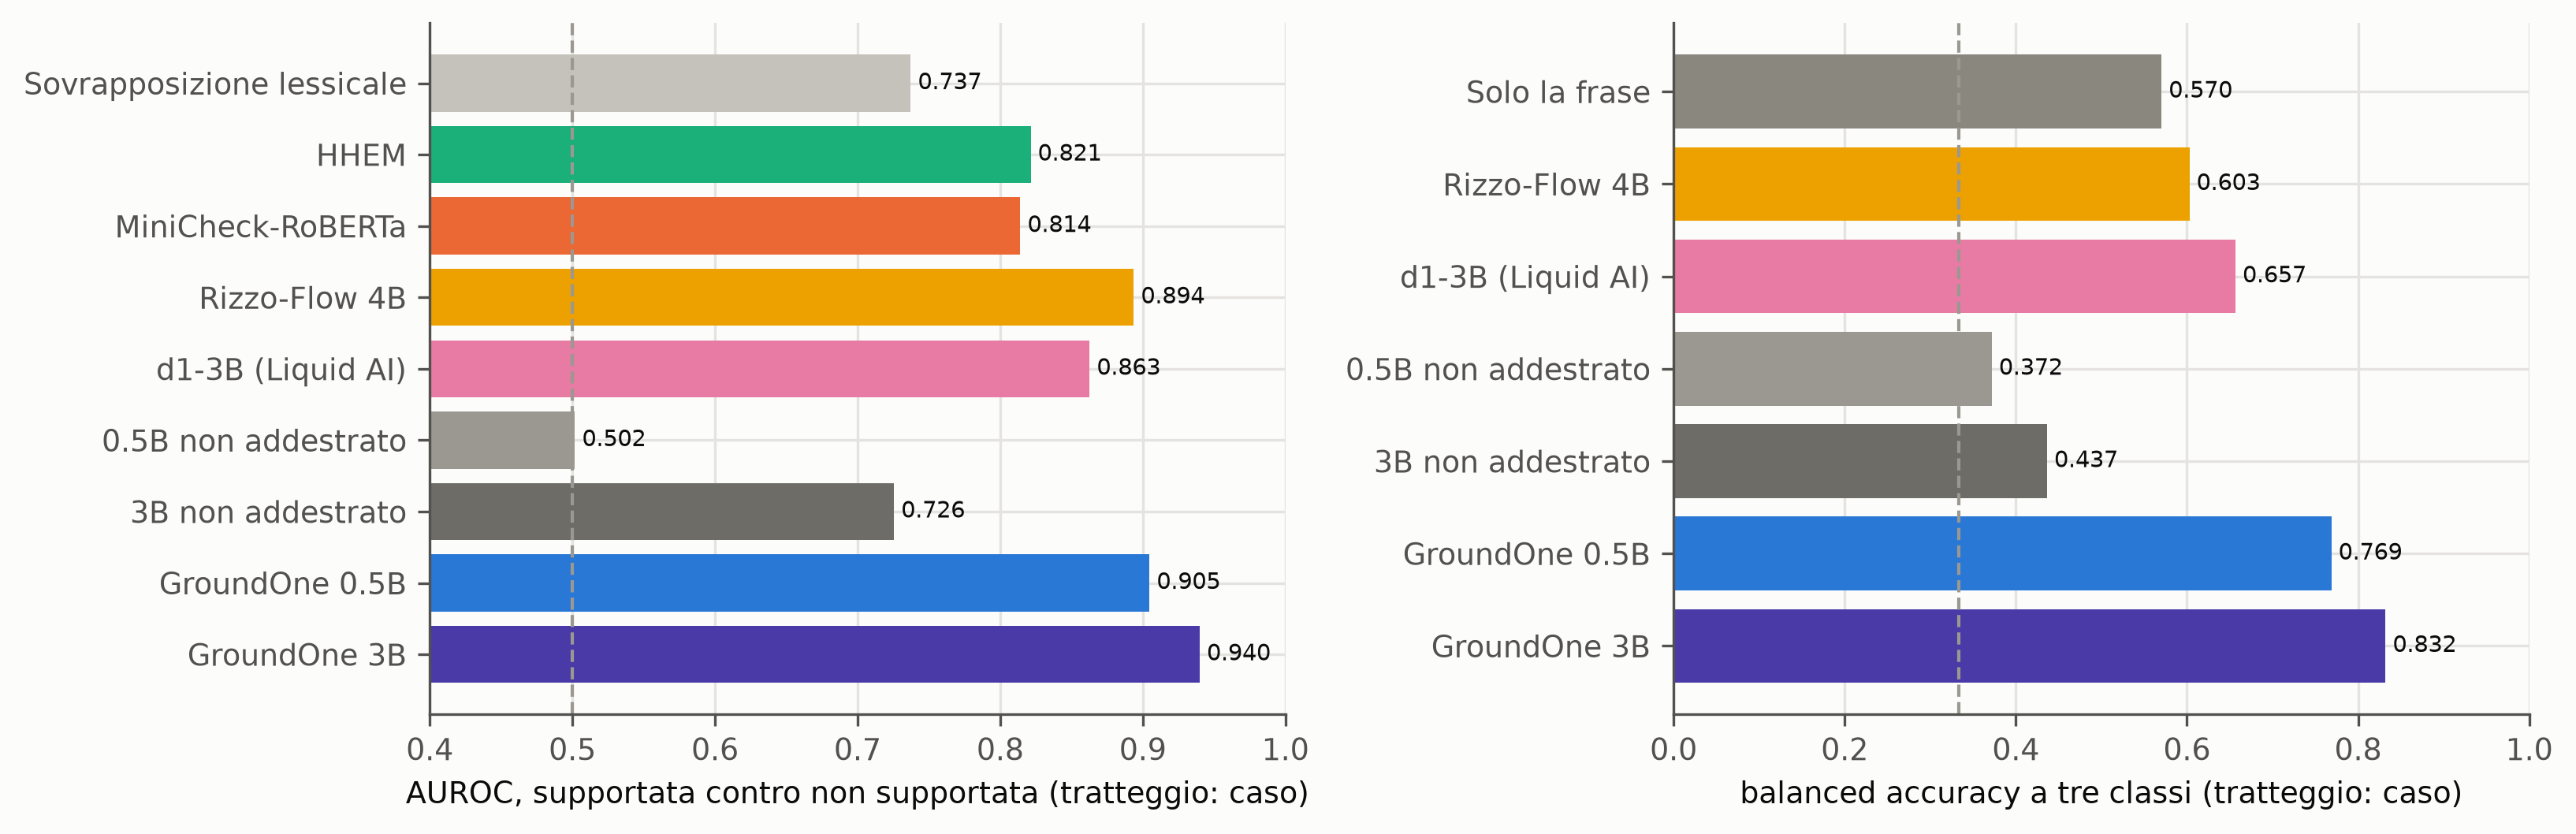
\includegraphics[width=\textwidth]{images/results/comparison_t1.png}
\caption{T1: AUROC di $P(\text{supported})$ per ogni sistema (a sinistra) e balanced accuracy a tre classi per i sistemi
con output a tre classi (a destra). Rizzo-Flow è valutato su 300 risposte e il 3B non addestrato su 600; tutti gli altri
sistemi, compreso il decision model generalista d1-3B, sull'intero test set.}
\label{fig:results-comparison}
\end{figure}

Il confronto più istruttivo è quello con il System One generalista. Sulle stesse 300 risposte di T1, Rizzo-Flow, un
modello da 4B sottoposto a fine-tuning per decisioni generiche, raggiunge una balanced accuracy a tre classi di 0.603,
contro 0.798 del GroundOne 0.5B e 0.840 del 3B; le differenze, $+0.195$ (da $+0.136$ a $+0.249$) e $+0.237$ (da
$+0.184$ a $+0.285$), sono ampie. Il suo AUROC (0.894) è vicino a quello del 0.5B su queste risposte (0.916; la
differenza non è significativa), perché ordina bene le frasi ma predice ``supportata'' per il 90\,\% di esse; il 3B le
ordina meglio ($+0.056$, da $+0.034$ a $+0.079$). Uno specialista otto volte più piccolo supera quindi il generalista
nella decisione per cui è stato progettato, e lo eguaglia nella capacità di ordinare le frasi.

Un decision model generalista della stessa dimensione offre la verifica più severa del valore della specializzazione,
perché d1-3B è già addestrato a prendere decisioni tipizzate e si differenzia da GroundOne soprattutto per i dati su cui
è stato addestrato. Sull'intero T1 raggiunge una balanced accuracy a tre classi di 0.657 e un AUROC di 0.863. Entrambi i
modelli GroundOne fanno nettamente meglio: il 0.5B, sei volte più piccolo, di $+0.112$ (da $+0.092$ a $+0.133$) nella
balanced accuracy a tre classi e di $+0.042$ in AUROC, il 3B di $+0.175$ (da $+0.157$ a $+0.195$) e di $+0.077$. Il
divario è massimo sulle risposte lunghe, dove d1-3B scende a 0.527 con quattordici o più decisioni mentre il GroundOne
3B resta a 0.839 ($+0.312$, da $+0.230$ a $+0.405$); inoltre d1-3B riconosce soltanto metà delle frasi non menzionate
(recall 0.49). Nel dominio delle risposte RAG, dunque, la specializzazione vale molto più di un addestramento generico a
prendere decisioni.

Su LLM-AggreFact (T2) il modello 0.5B raggiunge una balanced accuracy media macro di 70.1 sugli undici dataset, contro
64.2 dello stesso modello usato zero-shot e 72.8 del modello 7B zero-shot nella leaderboard pubblica. Resta sotto
MiniCheck-RoBERTa (74.0) di 3.9 punti, una differenza significativa. Sui quattro dataset più vicini alla
retrieval-augmented generation i due sono alla pari (74.4 contro 74.6), e nella colonna di RAGTruth GroundOne è in
vantaggio, 82.1 contro 76.5, in un confronto che lo favorisce perché è stato addestrato sulle risposte del training set
di RAGTruth. Al di fuori del RAG il 0.5B è inferiore all'encoder di sette-nove punti su AggreFact-CNN, AggreFact-XSum,
FactCheck-GPT e REVEAL: è il costo atteso di un addestramento sui soli dati RAG.

Il modello 3B, valutato sull'intero test set, colma gran parte di questo divario. La sua balanced accuracy media macro
è 74.8, alla pari con MiniCheck-RoBERTa (74.0; differenza appaiata $+0.8$ punti, intervallo da $-0.5$ a $+2.1$) e
superiore al punteggio zero-shot pubblicato per il modello 7B (72.8, per il quale non si può calcolare un intervallo).
Sui dataset RAG raggiunge 76.9, 2.4 punti sopra l'encoder (intervallo da $+1.4$ a $+3.3$). Il suo guadagno rispetto al
0.5B, $+4.7$ punti (da $+3.4$ a $+5.9$), è diffuso, con i miglioramenti maggiori su REVEAL, WiCE, FactCheck-GPT e XSum:
la dimensione del modello migliora quindi il trasferimento al di fuori del dominio di addestramento. Il 3B resta
nettamente sotto l'encoder soltanto nella summarization di notizie (AggreFact-CNN, 59.3 contro 67.1). Rizzo-Flow, sui
1{,}093 elementi del suo sottocampione, raggiunge 61.5, e su questi il GroundOne 3B fa meglio di 12.0 punti (da $+7.4$ a
$+16.5$). Una valutazione indipendente del System One closed Jev sullo stesso test set e con la stessa metrica riporta
78.6, e 76.9 per un modello open da 27B letto attraverso le lettere di risposta, con prompt diversi da quelli usati qui,
per cui non è possibile calcolare alcun intervallo~\cite{deusser2026jev}. Su un benchmark ampio di groundedness, quindi,
uno specialista da 3B addestrato soltanto su risposte RAG eguaglia il miglior encoder di piccole dimensioni, ma resta
sotto lo stato dell'arte closed e sotto modelli open molto più grandi. Il generalista d1-3B conferma il quadro a parità di
dimensione: su un sottocampione casuale di 4{,}000 elementi raggiunge 75.7, contro 74.3 del GroundOne 3B sugli stessi
elementi, una differenza non significativa ($-1.3$, da $-4.0$ a $+1.0$), mentre supera il 0.5B di 6.5 punti. È più
debole nella colonna di RAGTruth (78.9 contro 87.3) e nettamente più forte su WiCE e sulla summarization di dialoghi.

\section{Trasferimento a un dominio diverso (T3)}
\label{sec:results-t3}

Su VitaminC il quadro si rovescia. Sull'intero test set il 0.5B raggiunge una balanced accuracy a tre classi di 0.442 e
il 3B di 0.527, con AUROC di 0.722 e 0.817, mentre MiniCheck-RoBERTa arriva a un AUROC di 0.968. Sulle 600 coppie
valutate con Rizzo-Flow, il modello generalista ottiene 0.712 e un AUROC di 0.909, contro 0.442 e 0.744 del 0.5B e 0.537
e 0.845 del 3B. Due fatti aiutano a interpretare questi numeri. MiniCheck-RoBERTa parte dal modello AlignScore, i cui
dati di addestramento comprendono VitaminC~\cite{zha2023alignscore}: T3 appartiene quindi alla sua distribuzione di
addestramento, mentre per GroundOne misura il trasferimento da RAGTruth. Inoltre, il guadagno del 3B sul 0.5B in T3 si
deve alla dimensione del modello più che all'addestramento su dati RAG: il 3B non addestrato raggiunge già 0.531 e un
AUROC di 0.821. Il decision model generalista della stessa dimensione rende esplicito il contrasto: d1-3B raggiunge
0.724 e un AUROC di 0.913 sull'intero T3, davanti al GroundOne 3B di 0.197 e 0.096, l'esatto opposto di quanto accade su
T1. La specializzazione su risposte RAG migliora quindi in modo sostanziale il task RAG, ma non basta, da sola, a
produrre un fact checker generale. La Sezione~\ref{sec:results-errors} mostra quali casi sfuggono.

\section{Readout e generazione a confronto}
\label{sec:results-readout}

Il controllo B2 isola il contributo del readout. A parità di pesi ottenuti con il fine-tuning, di prompt e di singolo
forward pass, il verdetto a ogni marker viene letto dalle tre lettere di risposta, come fa GroundOne, oppure preso come il
token che emetterebbe la generazione greedy (Figura~\ref{fig:results-readout}). Per il 0.5B il token generato dà una
balanced accuracy a tre classi di 0.521 contro 0.769 del readout, una differenza di $+0.248$ (da $+0.228$ a $+0.269$):
in un quarto dei marker (24.7\,\%) il modello non emetterebbe affatto una lettera, ma per lo più un semplice spazio,
l'inizio di una risposta più lunga. Per il 3B il token generato è quasi sempre una lettera (1.2\,\% di errori di formato)
e concorda con il readout nel 92\,\% dei marker, eppure il readout resta migliore, 0.832 contro 0.761 ($+0.071$, da
$+0.059$ a $+0.083$). Sulle risposte con quattordici o più decisioni il divario è massimo per il modello piccolo,
$+0.346$.

\begin{figure}[htbp]
\centering
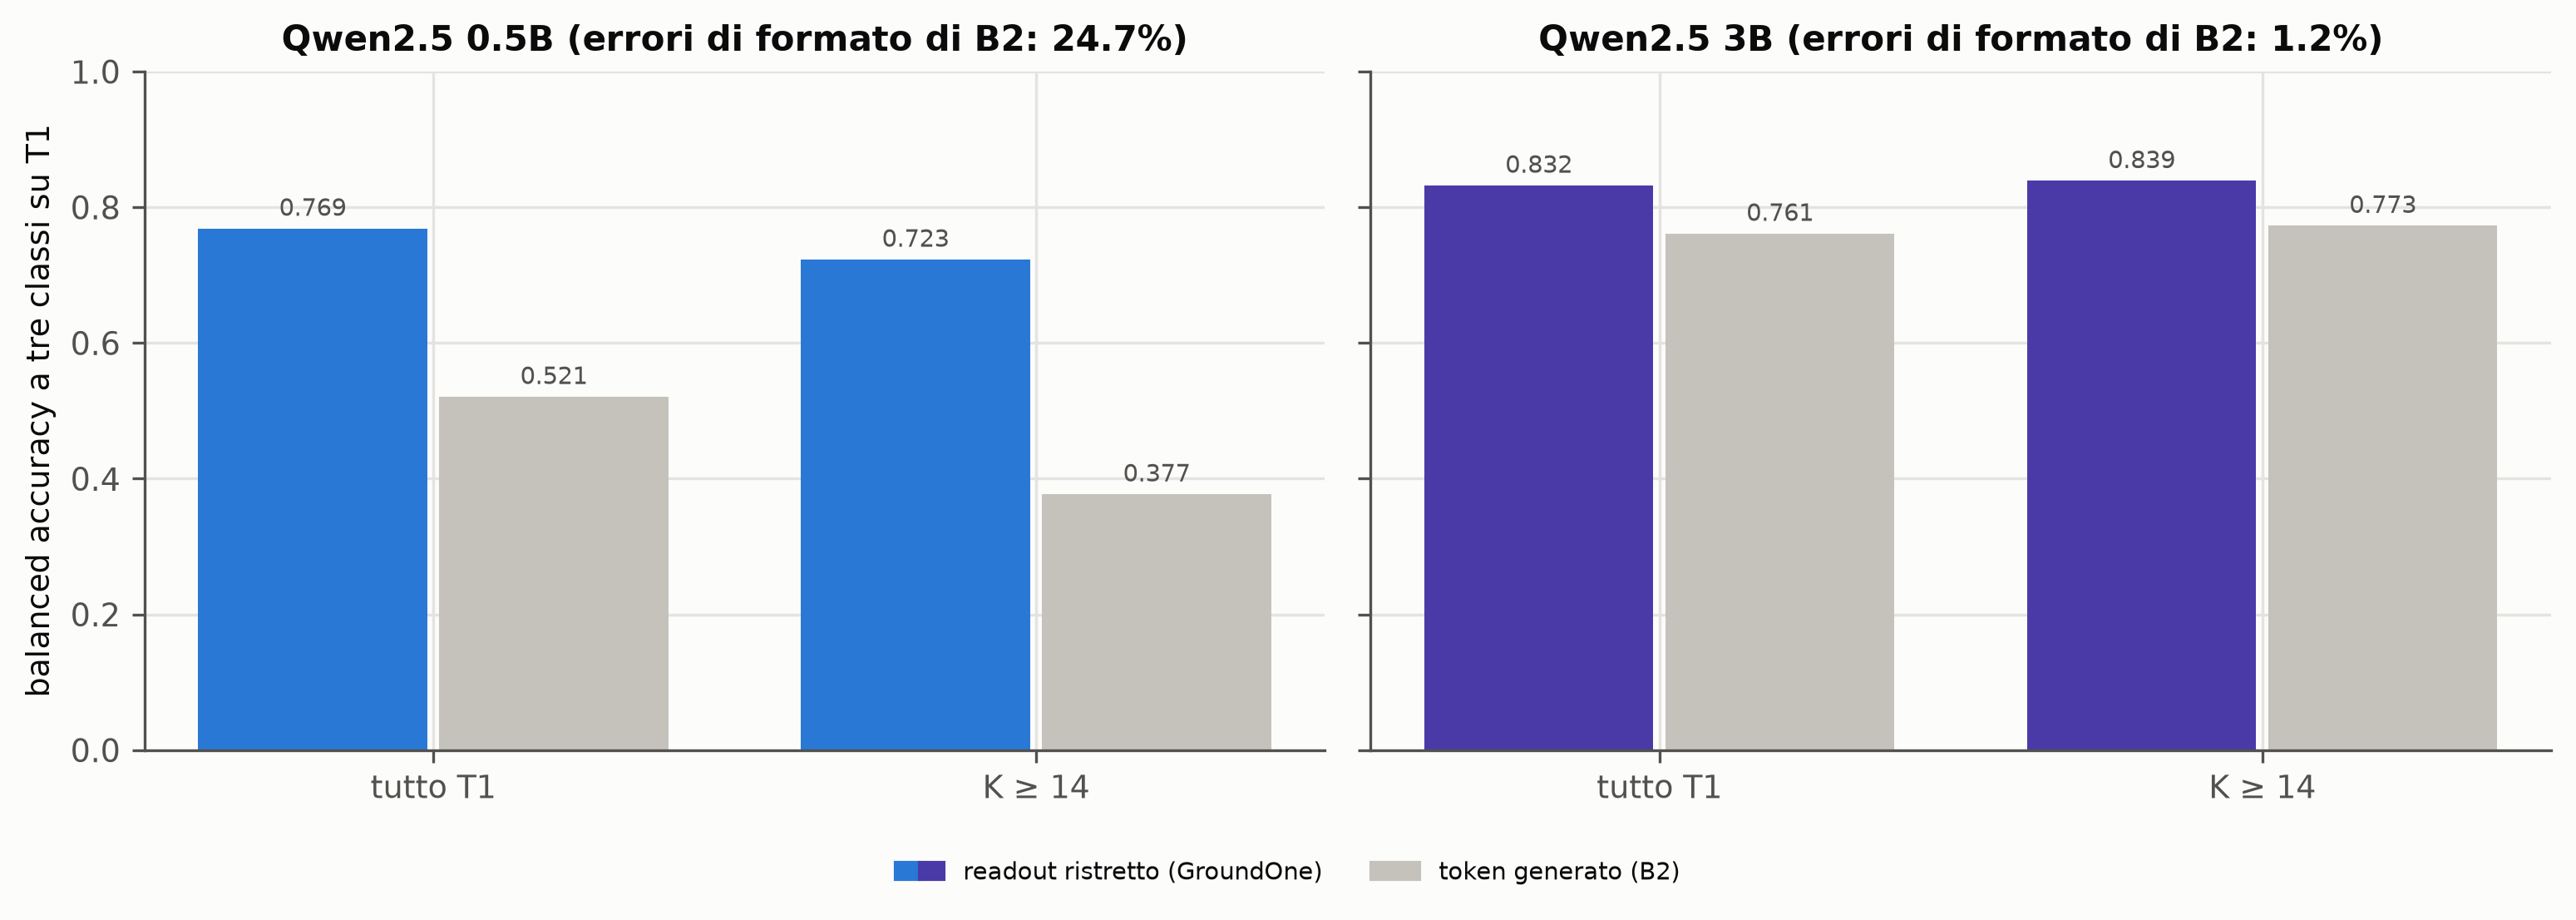
\includegraphics[width=\textwidth]{images/results/readout_vs_generation.png}
\caption{Controllo B2 sull'intero T1: con gli stessi pesi e lo stesso forward pass, il verdetto è letto dalle tre lettere
di risposta (GroundOne) oppure preso come il token che emetterebbe la generazione greedy (gli errori di formato sono
contati come errori).}
\label{fig:results-readout}
\end{figure}

Le due opzioni hanno la stessa latenza, perché entrambe richiedono un solo forward pass; a cambiare è la regola di
decisione. Restringere la scelta alle opzioni ammissibili elimina per costruzione gli errori di formato e, poiché il
modello è addestrato soltanto a ordinare le tre lettere, fornisce anche la decisione più accurata
(Sezione~\ref{sec:method-readout}). Più il modello è piccolo, più questa restrizione conta. L'idea, spesso ripetuta, che
leggere i logit delle risposte e generare un singolo token di risposta siano equivalenti vale dunque per il costo, ma
non per l'accuratezza di un verificatore sottoposto a fine-tuning.

\section{Calibrazione e selective prediction}
\label{sec:results-calibration}

Le probabilità grezze sottostimano il supporto. Nel reliability diagram (Figura~\ref{fig:results-reliability}) la curva
grezza giace sopra la diagonale, perché i pesi delle classi addestrano il modello come se le classi fossero bilanciate;
l'ECE binario su T1 è 0.30 per il 0.5B e 0.18 per il 3B. La temperatura e il bias stimati sul dev set portano l'ECE su
T1 a 0.019 per entrambi i modelli, e a 0.020 per la seconda esecuzione del 0.5B, e riducono la negative log-likelihood
da 0.55 a 0.21 (0.5B) e da 0.36 a 0.17 (3B), lasciando l'AUROC praticamente invariato. La mappa stimata sul dev set si
trasferisce quindi al test set dello stesso dominio.

\begin{figure}[htbp]
\centering
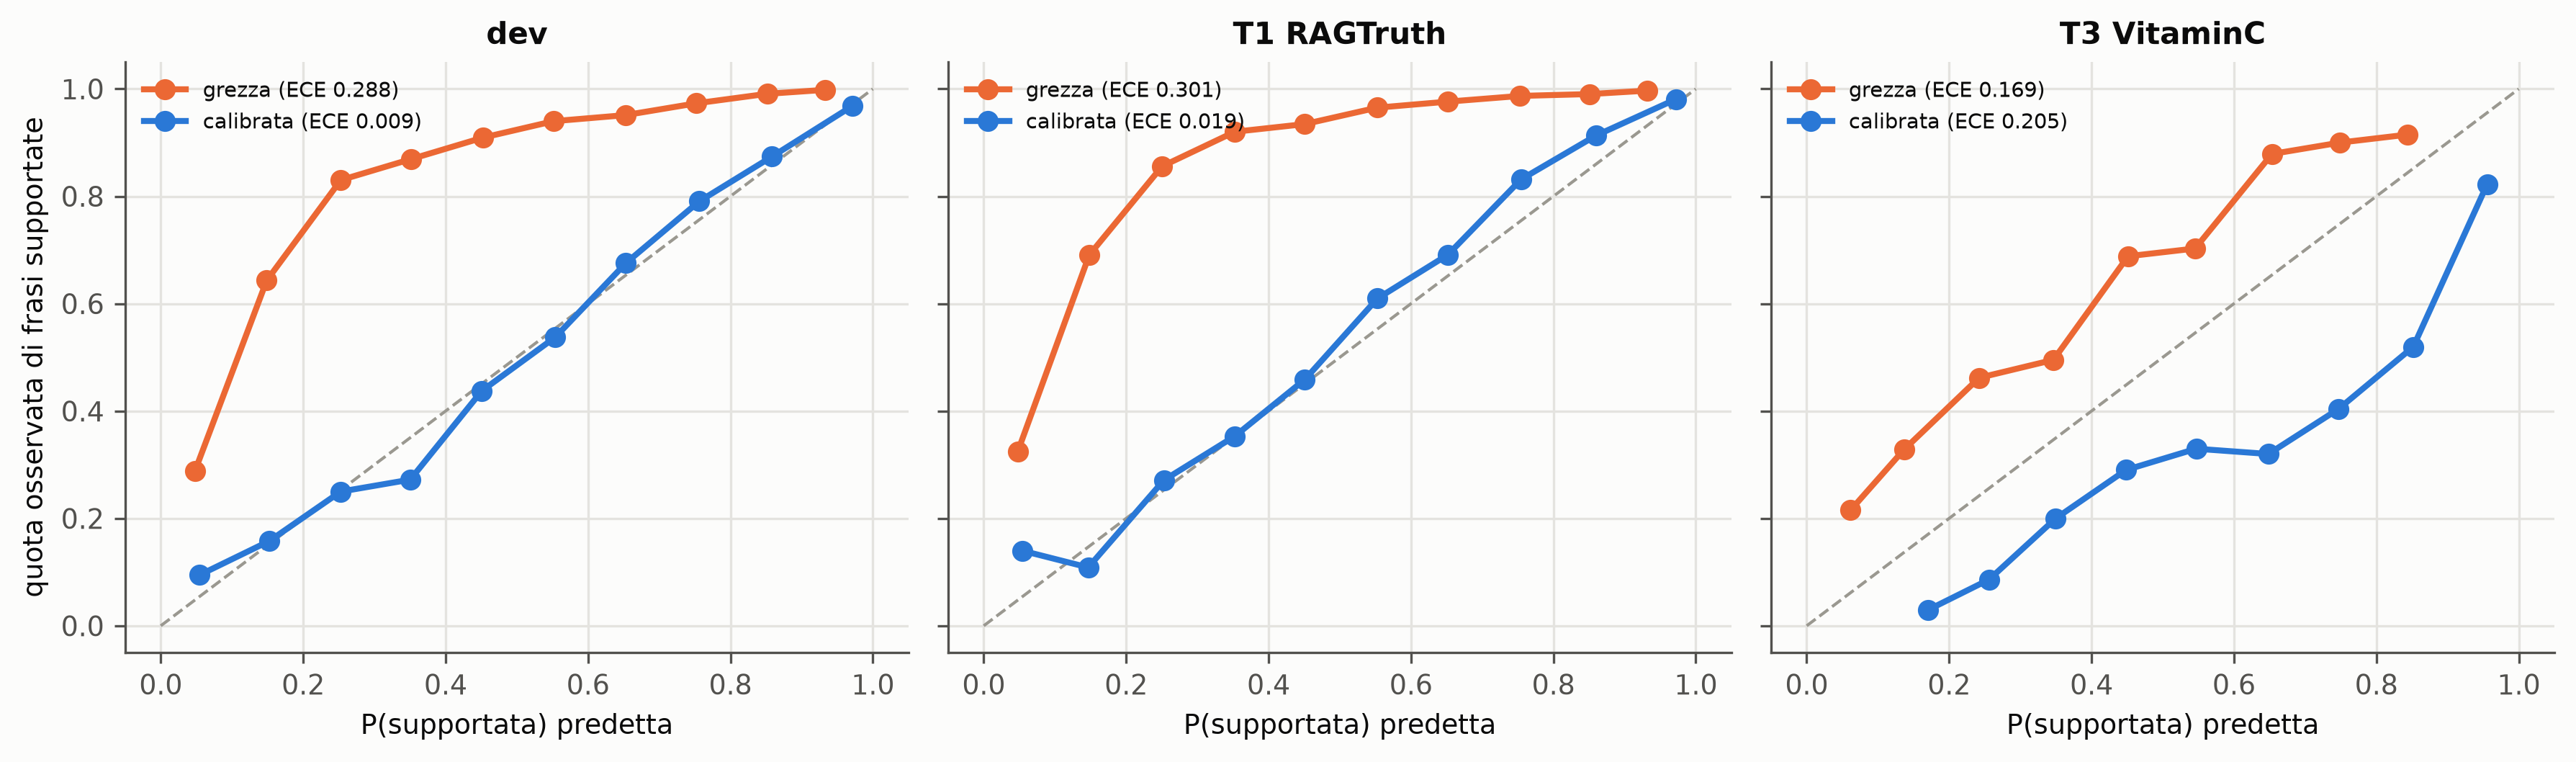
\includegraphics[width=\textwidth]{images/results/g1-05b-reliability.png}
\caption{Reliability diagram di $P(\text{supported})$ del 0.5B prima (grezza) e dopo la calibrazione sul dev set, per il
dev set, T1 e T3. I punti corrispondono a intervalli con almeno 20 frasi.}
\label{fig:results-reliability}
\end{figure}

La calibrazione ha però una conseguenza da tenere presente. Il bias ripristina la frequenza reale di ciascuna classe,
per cui la classe calibrata più probabile diventa più spesso ``supportata'': per il 0.5B su T1 l'accuratezza sale da
0.82 a 0.93, ma la balanced accuracy a tre classi scende da 0.77 a 0.63. Scegliere la classe calibrata più probabile non
è quindi una buona regola di decisione quando i tre tipi di errore hanno lo stesso peso. La regola con cui vengono
restituite le etichette, descritta nella Sezione~\ref{sec:method-calibration}, risolve il problema: con la soglia
stimata sul dev set, $\tau$ = 0.935 per il 0.5B, 0.895 per la sua seconda esecuzione e 0.925 per il 3B, raggiunge 0.758,
0.769 e 0.830 su T1, entro 0.01 dalla decisione grezza valutata in tutto il capitolo, e mantiene coerenti etichette e
probabilità calibrate. Le soglie sono alte perché il 91\,\% delle frasi di RAGTruth è supportato: una frase viene
restituita come supportata soltanto quando il modello è molto sicuro.

Usate come confidenze, le probabilità calibrate rendono efficace la selective prediction: rinviare le frasi su cui il
modello è meno sicuro riduce rapidamente il tasso di errore della decisione binaria, con un'area sotto la curva
risk--coverage di 0.015 (0.5B) e 0.010 (3B) su T1 (Figura~\ref{fig:results-risk}).

\begin{figure}[htbp]
\centering
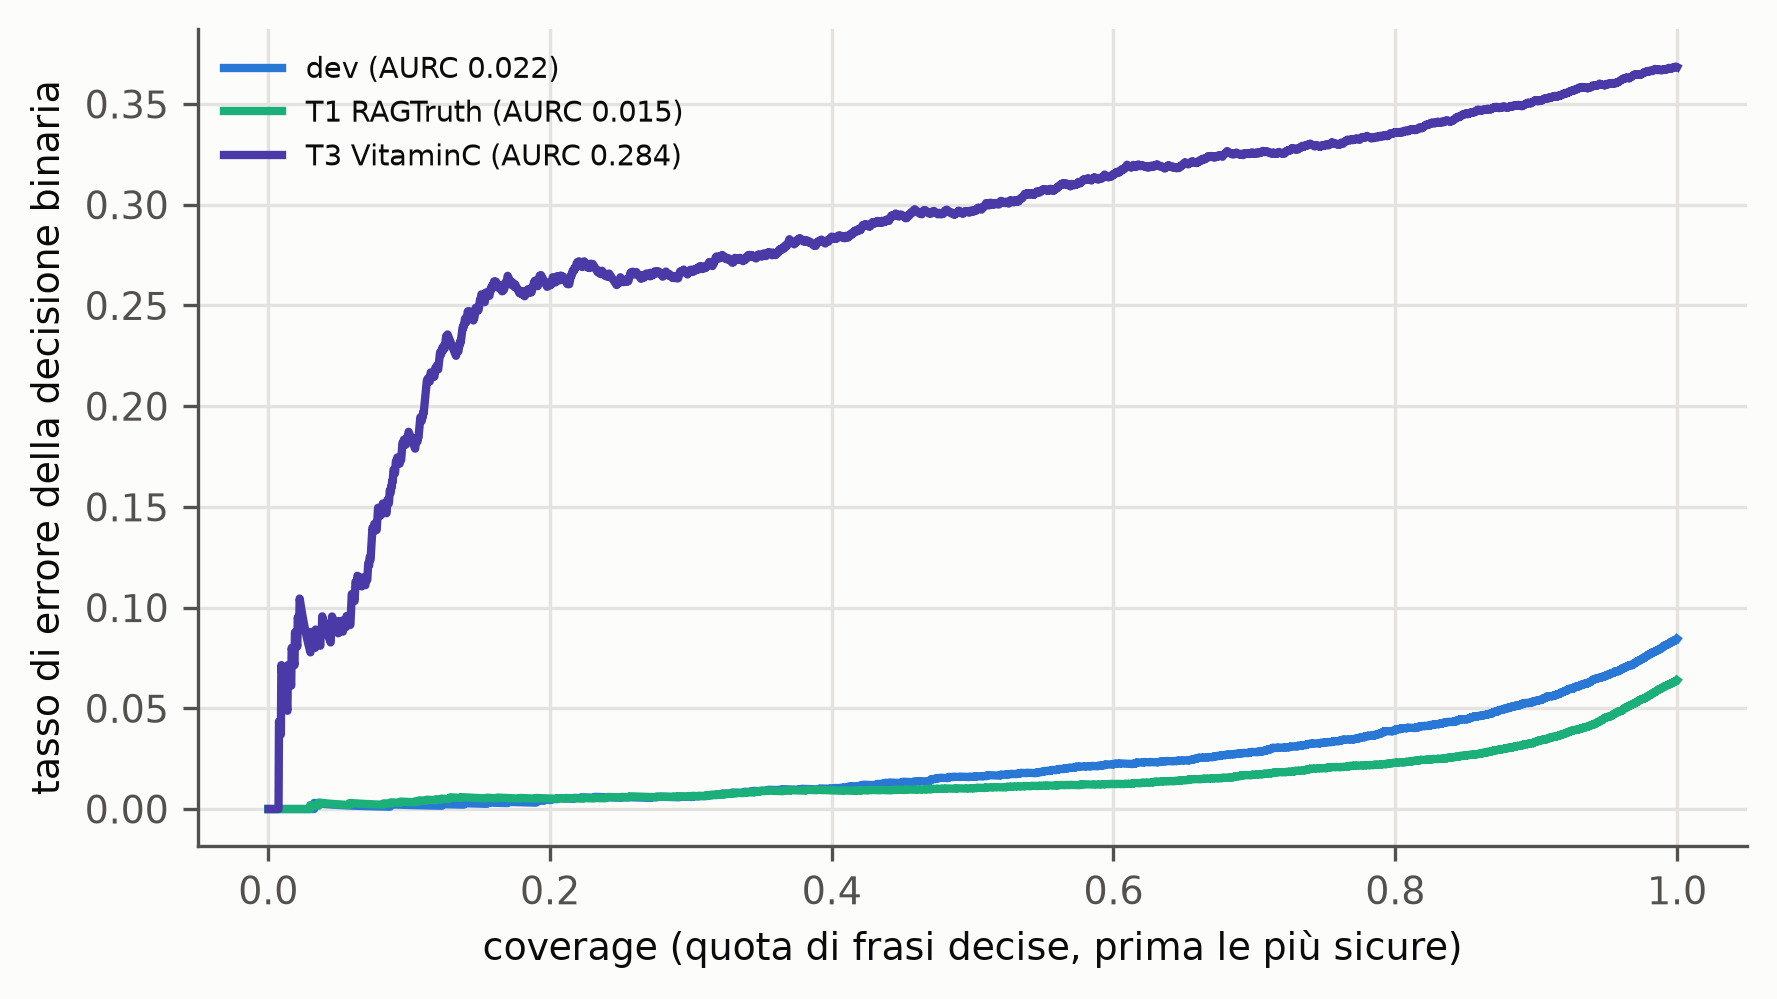
\includegraphics[width=0.75\textwidth]{images/results/g1-05b-risk_coverage.png}
\caption{Curve risk--coverage della decisione binaria del 0.5B con probabilità calibrate: tasso di errore al crescere
delle frasi meno sicure che vengono rinviate.}
\label{fig:results-risk}
\end{figure}

La calibrazione non si trasferisce a VitaminC, dove l'ECE binario sale da 0.17 a 0.21 per il 0.5B e da 0.14 a 0.19 per
il 3B, e dove la regola di restituzione perde 0.02--0.04 rispetto alla decisione grezza. Il bias codifica il tasso di
base di RAGTruth, mentre VitaminC è bilanciato per costruzione. Una calibrazione vale per la distribuzione su cui è stata
stimata, per cui ogni impiego reale richiede un piccolo campione etichettato dei propri dati.

\section{Probabilità a parità di output}
\label{sec:results-equal-output}

I giudici a parità di output servono a stabilire se un giudice generativo della stessa dimensione, a cui si chiede lo
stesso contenuto di GroundOne, possa eguagliare la qualità delle sue probabilità. La risposta è negativa
(Figura~\ref{fig:results-equal}). Sulle 200 risposte del sottoinsieme di latenza, con tutti i sistemi calibrati allo
stesso modo sul dev set, l'AUROC di $P(\text{supported})$ è 0.94 e 0.97 per GroundOne, 0.48 e 0.68 per il giudice le cui
probabilità sono lette dai logit, e 0.47 e 0.58 per il giudice che le scrive, rispettivamente per il 0.5B e per il 3B.
L'area sotto la curva risk--coverage è 0.009 e 0.005 per GroundOne, contro valori da 0.048 a 0.063 per i giudici, da
cinque a dodici volte maggiori. L'accuratezza delle decisioni segue lo stesso andamento: 0.835 e 0.900 per GroundOne,
al massimo 0.41 per qualsiasi giudice.

\begin{figure}[htbp]
\centering
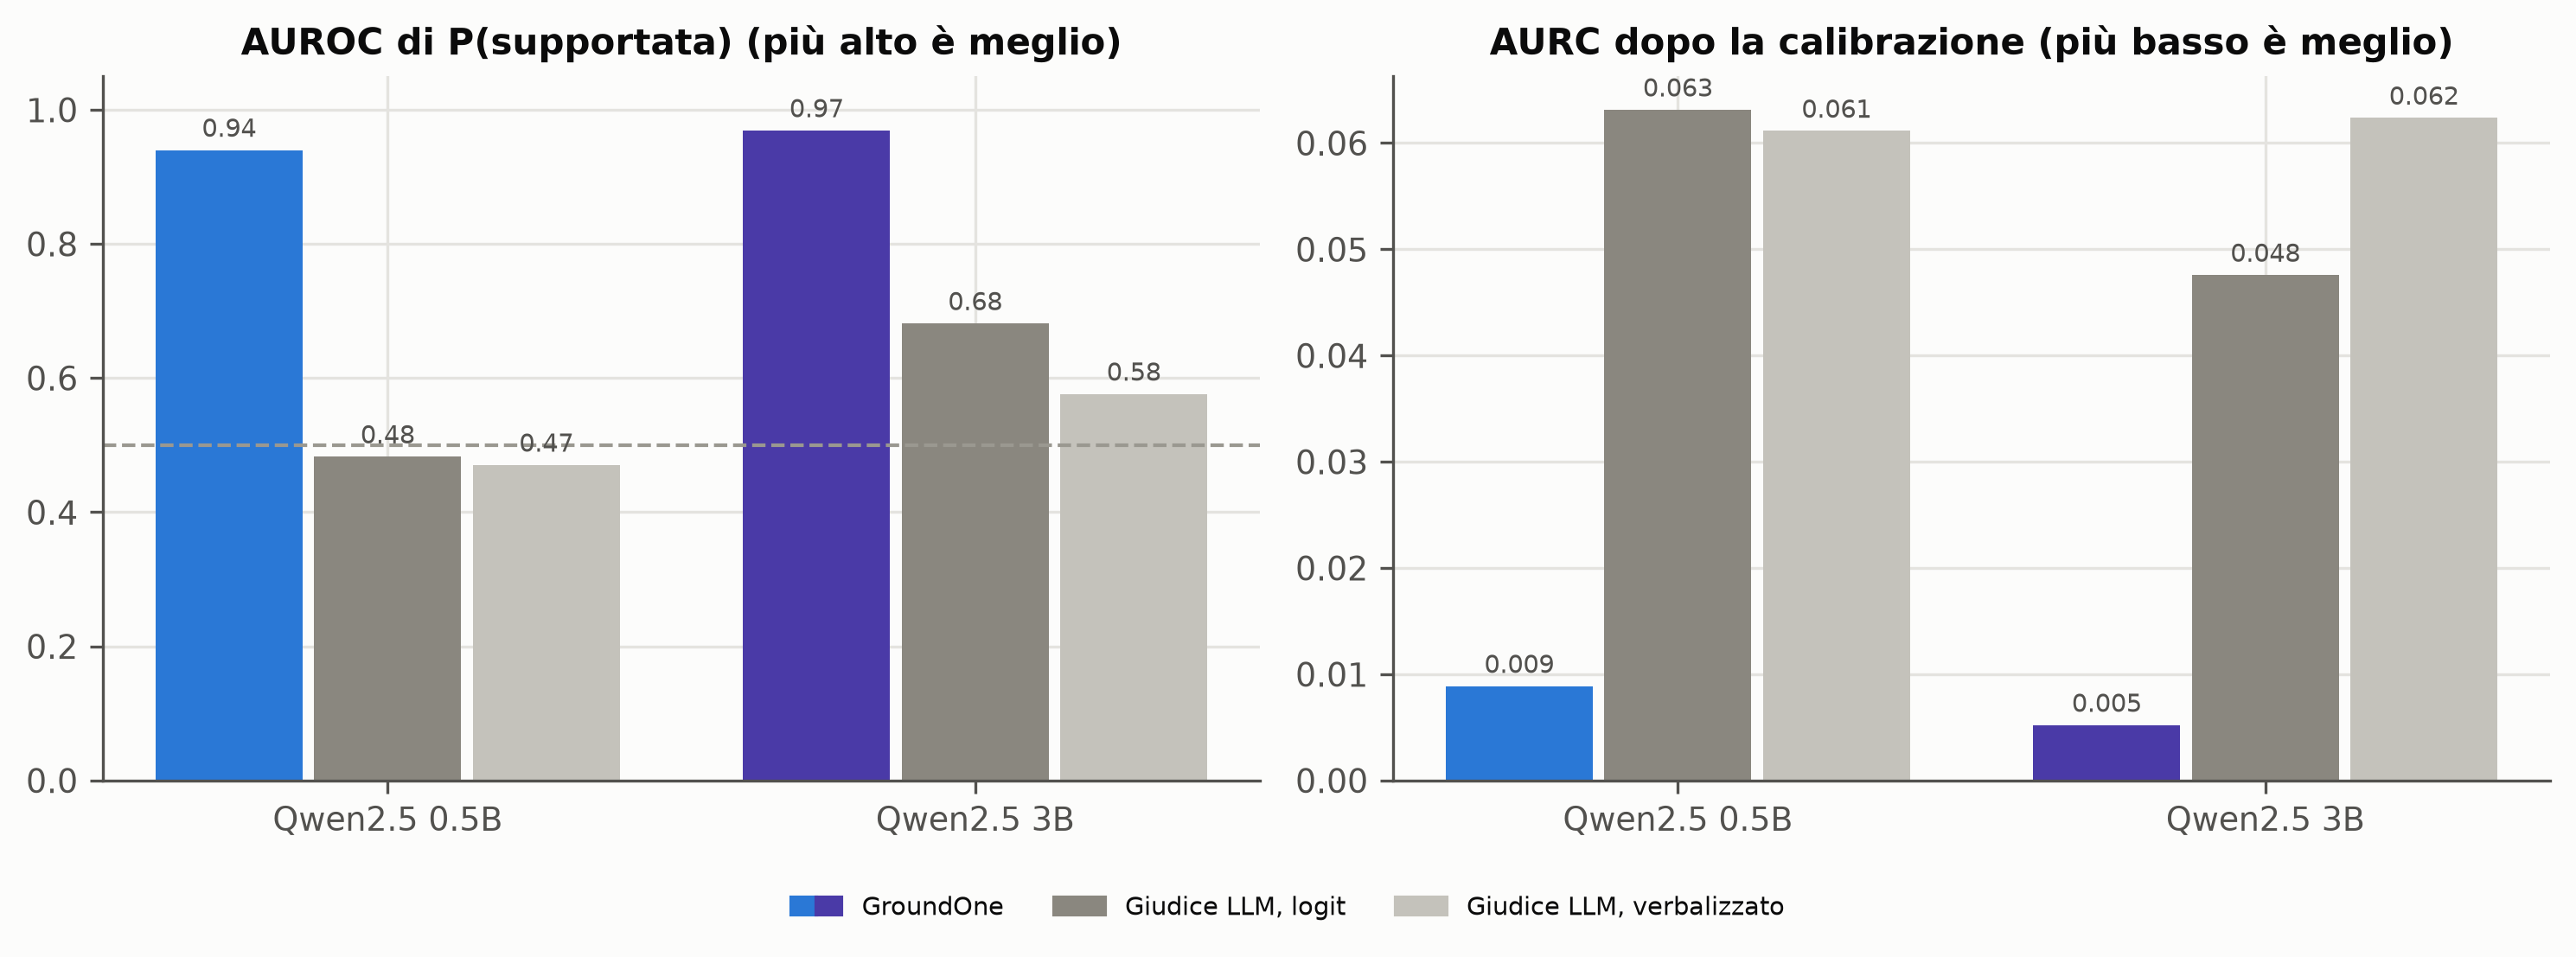
\includegraphics[width=\textwidth]{images/results/equal_output_judges.png}
\caption{Confronto a parità di output sulle 200 risposte di latenza: giudici generativi della stessa dimensione a cui si
chiede l'output di GroundOne, con probabilità lette dai logit della lettera generata oppure scritte in JSON; tutti i
sistemi sono calibrati sul dev set con la stessa mappa. Solo frasi con un verdetto valido.}
\label{fig:results-equal}
\end{figure}

Altre due osservazioni contano nella pratica. Le probabilità scritte a parole non portano quasi alcuna informazione: il
3B scrive un vettore con tutta la massa su una sola classe per il 93\,\% delle frasi, usando appena sedici vettori
distinti, e il 0.5B scrive pareggi non informativi, come probabilità uguali per tutte le classi; contando come errori i
pareggi privi di etichetta, la sua balanced accuracy scende da 0.234 a 0.081. Il dato concorda con l'osservazione che la
confidenza verbalizzata dei modelli piccoli è grossolana e poco informativa~\cite{xiong2024uncertainty,tian2023justask}.
Inoltre, l'ECE da solo nasconderebbe tutto ciò: dopo la calibrazione ogni sistema, giudici compresi, ottiene un ECE
binario compreso tra 0.03 e 0.05, perché una mappa di calibrazione può allineare la confidenza media al tasso di base
anche quando le probabilità non separano le classi. La capacità discriminativa va misurata a parte, con l'AUROC e con la
curva risk--coverage.

Chiedere le probabilità, infine, ha un costo. Il giudice che le legge dai logit è veloce quanto il giudice sintetico,
perché genera le stesse lettere, mentre il giudice che scrive l'oggetto JSON impiega sul 3B 17.0 secondi per risposta
con quattordici o più decisioni, quanto il giudice verboso, per un'accuratezza non superiore a quella del giudice
sintetico.

\section{Latenza in funzione di K}
\label{sec:results-latency}

La Figura~\ref{fig:results-latency} riporta la misura centrale della tesi: il tempo necessario per verificare una
risposta, sulle stesse 200 risposte di T1, al crescere del numero di decisioni. Tra i sistemi eseguiti in-process su MLX,
GroundOne è il più veloce a entrambe le dimensioni e in ogni fascia di $K$, e il suo vantaggio aumenta con $K$. Per le
risposte con quattordici o più decisioni il GroundOne 0.5B impiega 0.41 secondi, contro 0.80 del giudice sintetico e
2.51 del giudice verboso della stessa dimensione: è 1.95 volte più veloce del primo (da 1.82 a 2.14) e 6.16 volte più
veloce del secondo (da 5.72 a 6.67). Il GroundOne 3B impiega 2.57 secondi, contro 4.44 e 15.86, ed è quindi 1.73 volte
(da 1.65 a 1.82) e 6.18 volte (da 5.88 a 6.65) più veloce. Leggere tutti i verdetti in un unico forward pass è anche più
rapido che porre una domanda per frase in un batch, di un fattore 1.4--1.5 ai valori più alti di $K$. L'altra leva è la
dimensione del modello: il GroundOne 0.5B verifica una risposta circa sei volte più in fretta del 3B (0.33 contro 1.99
secondi in mediana).

\begin{figure}[htbp]
\centering
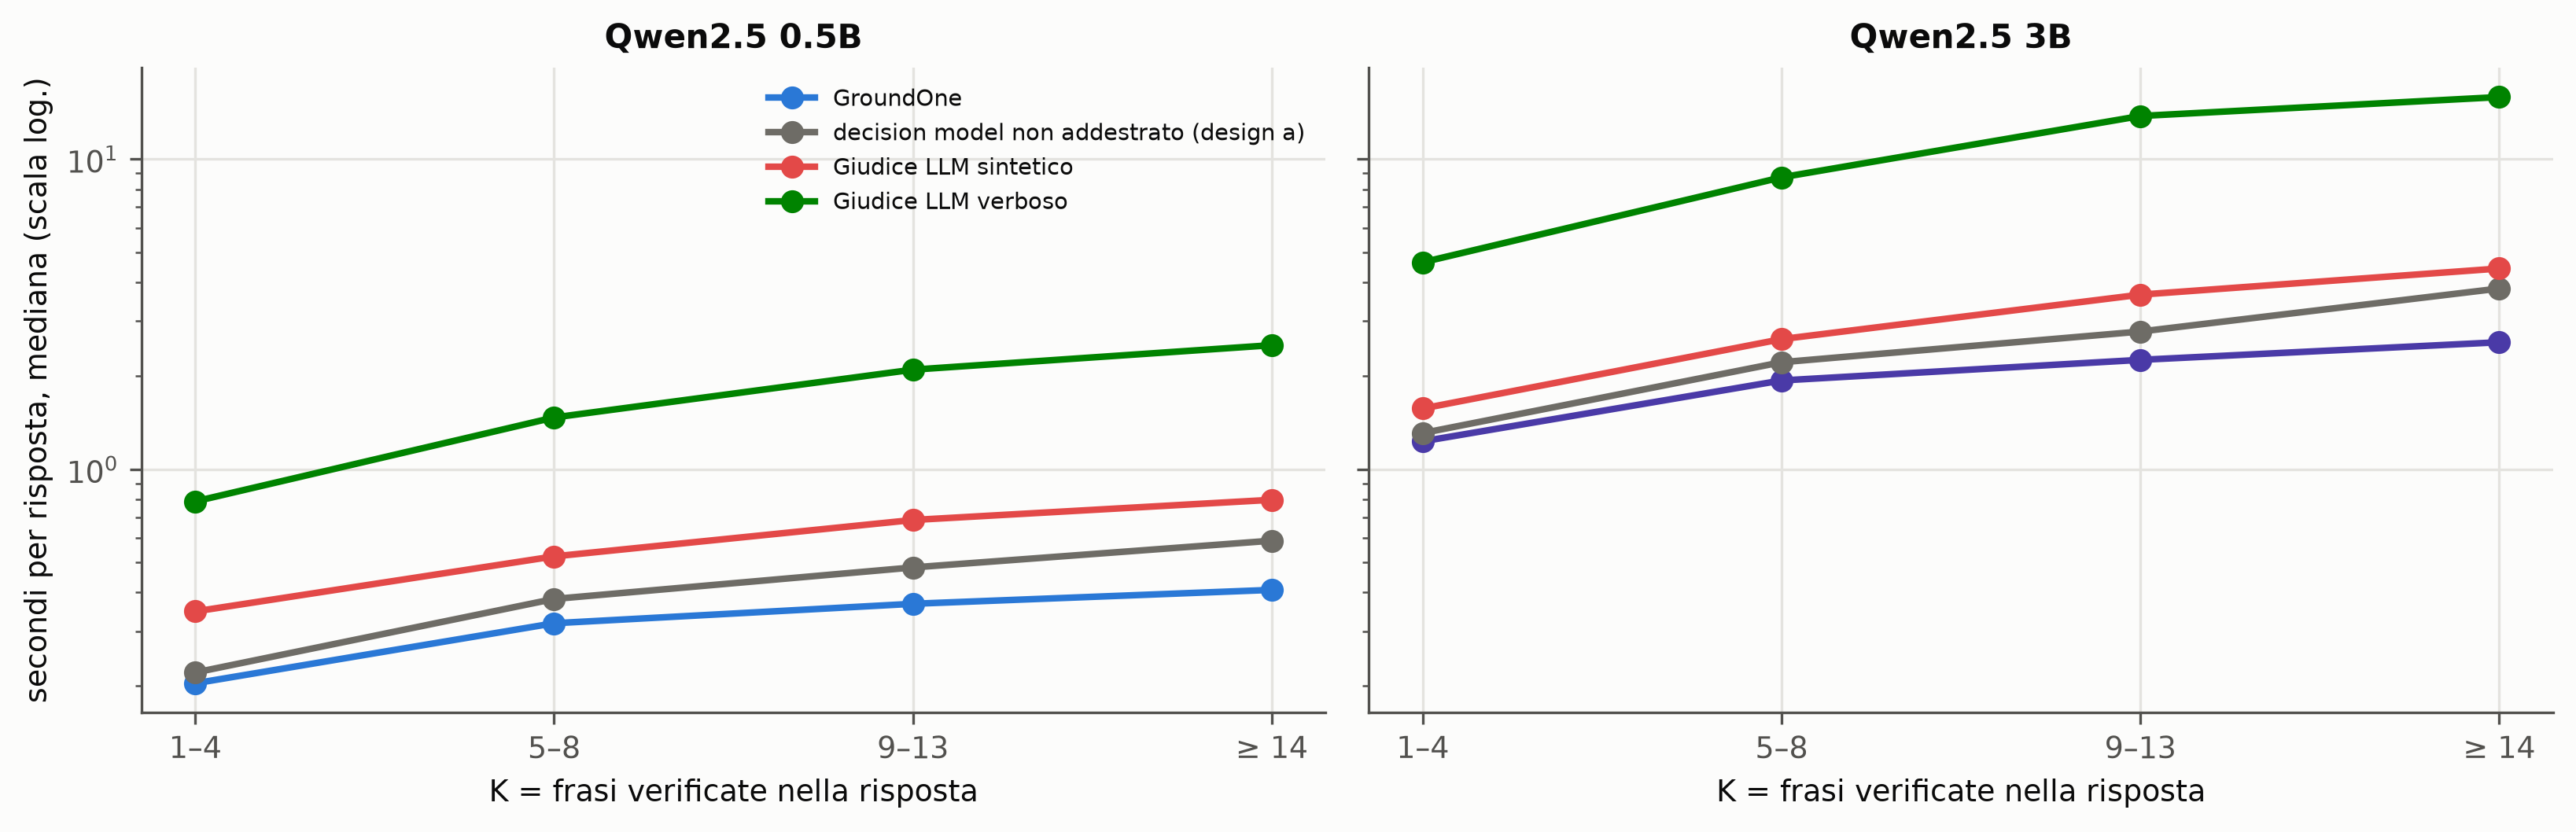
\includegraphics[width=\textwidth]{images/results/latency_vs_K.png}
\caption{Tempo mediano per risposta in funzione di $K$ sulle stesse 200 risposte di T1 (MLX in-process, una risposta
alla volta, M4 con 16\,GB), per GroundOne, il System One con una domanda per frase e i giudici generativi sintetico e
verboso. Scala logaritmica.}
\label{fig:results-latency}
\end{figure}

La velocità non è l'unica differenza (Figura~\ref{fig:results-judges}). I giudici generativi non addestrati sono anche
molto meno accurati e non sempre rispettano il formato di output. Il giudice verboso 0.5B produce un verdetto
interpretabile soltanto per il 3\,\% delle frasi, perché per lo più ricopia la risposta, e il giudice sintetico 0.5B
fallisce sul 23\,\%. I giudici 3B rispettano il formato molto meglio (0.1\,\% e 7.6\,\% di errori di formato), ma si
fermano a una balanced accuracy a tre classi di circa 0.40, contro 0.90 del GroundOne 3B sulle stesse risposte. Il
giudice verboso 3B scrive in media 248 token per risposta, che vanno tutti generati prima di poter usare il verdetto,
mentre GroundOne non ne genera nessuno.

\begin{figure}[htbp]
\centering
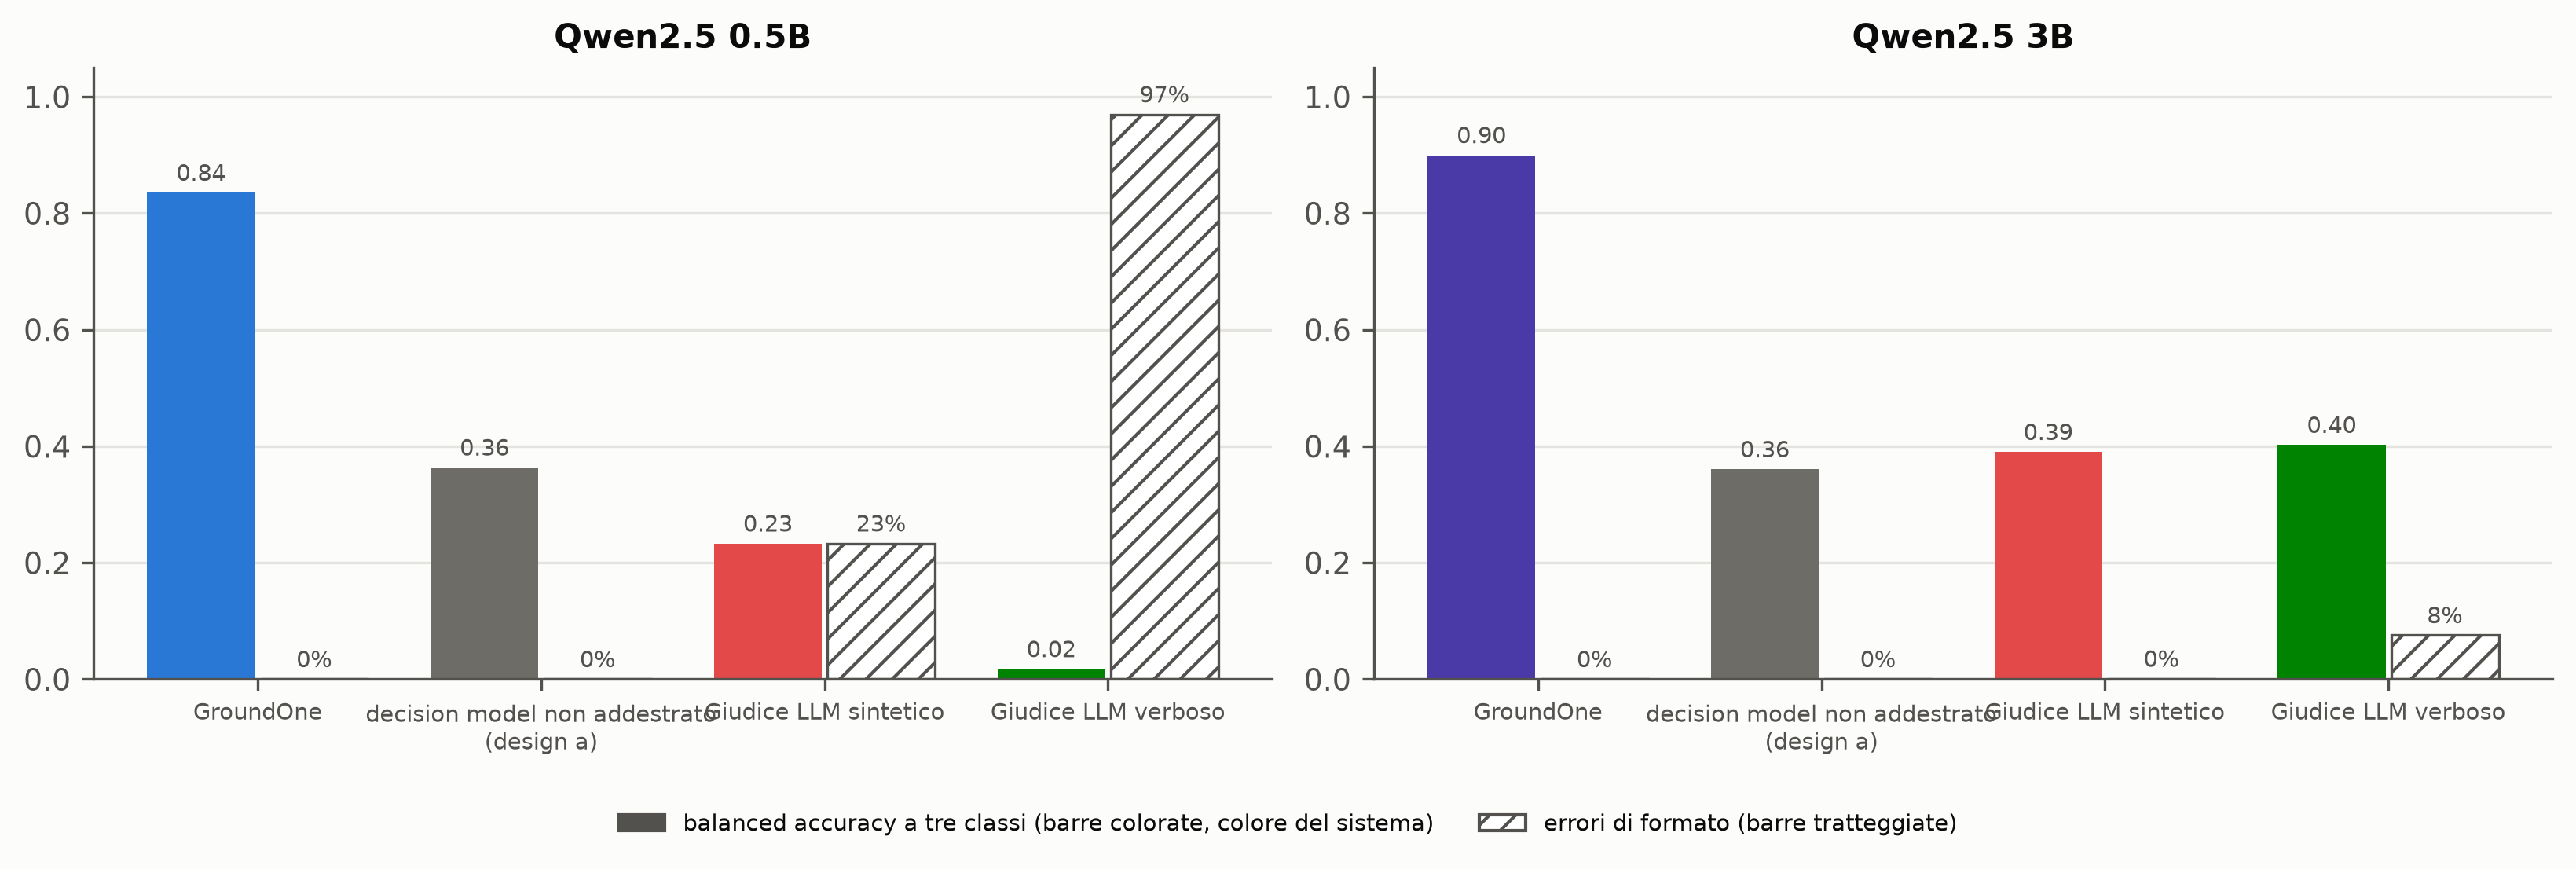
\includegraphics[width=\textwidth]{images/results/judges_quality_failures.png}
\caption{Sul sottoinsieme di latenza: balanced accuracy a tre classi (gli errori di formato sono contati come errori) e
quota di frasi il cui verdetto non è stato possibile interpretare.}
\label{fig:results-judges}
\end{figure}

\section{Energia per verifica}
\label{sec:results-energy}

La misura dell'energia introduce una precisazione che la sola latenza nasconde (Figura~\ref{fig:results-energy}).
GroundOne è il sistema che consuma meno energia a entrambe le dimensioni: 5.5 joule per risposta con il 0.5B e 33 con il
3B, contro 8.9 e 43 del giudice sintetico e 22.5 e 112 del giudice verboso. Il suo vantaggio, tuttavia, è minore di
quello sul tempo: 1.6 e 1.3 volte meno energia del giudice sintetico, 4.1 e 3.4 volte meno del verboso. Il motivo è la
potenza assorbita durante il calcolo. GroundOne trascorre il suo tempo in un unico, lungo prefill, che tiene la GPU
pienamente occupata e assorbe circa 16\,W oltre la potenza a riposo, mentre il decoding autoregressivo è limitato dalla
banda di memoria e assorbe 11--14\,W, ma per un tempo molto più lungo. È il comportamento atteso dalle due fasi
dell'inferenza dei transformer~\cite{patel2024splitwise}, e implica che uno speed-up non vada mai letto come un
risparmio di energia equivalente~\cite{samsi2023words,luccioni2024power}.

\begin{figure}[htbp]
\centering
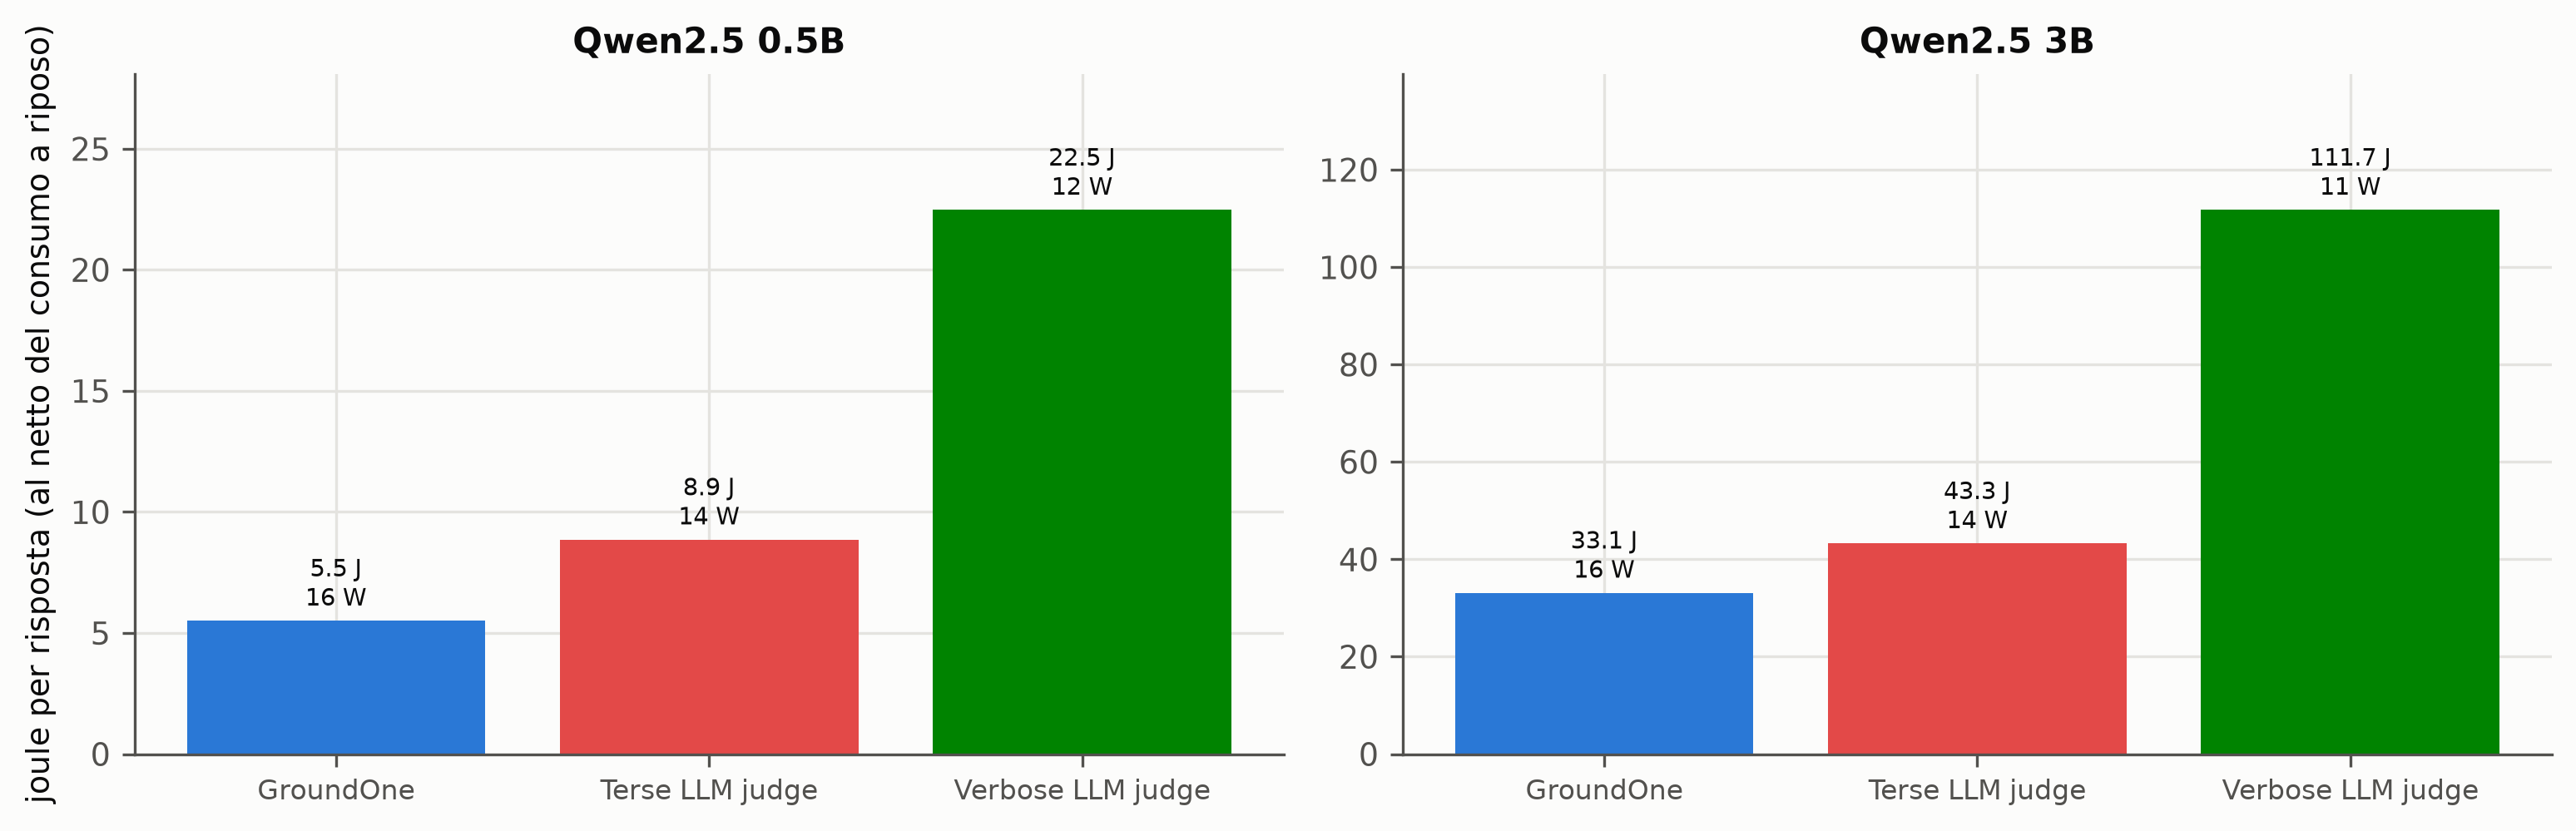
\includegraphics[width=\textwidth]{images/results/energy_per_answer.png}
\caption{Energia per risposta verificata su 100 risposte di latenza (powermetrics, CPU, GPU e Neural Engine, al netto
della potenza a riposo), con la potenza netta media durante l'esecuzione.}
\label{fig:results-energy}
\end{figure}

In termini assoluti i valori sono piccoli: 5.5 joule corrispondono a circa 0.0015 wattora, per cui il GroundOne 0.5B
potrebbe verificare circa seicento risposte con l'energia di un wattora, interamente sul portatile.

\section{Analisi degli errori}
\label{sec:results-errors}

Il risultato debole su VitaminC e le contraddizioni mancate su T1 hanno una causa comune, che la sovrapposizione
lessicale mette in evidenza. Su VitaminC, quando un'affermazione supportata condivide poche parole con la propria
evidenza (sovrapposizione inferiore a 0.4), il 0.5B la riconosce soltanto nel 2\,\% dei casi, contro il 64\,\% quando la
sovrapposizione supera 0.7, e non riconosce mai una contraddizione in un'affermazione priva di cifre. I modelli si
appoggiano in parte alla sovrapposizione lessicale: un'affermazione parafrasata sembra ``non menzionata'', mentre una
piccola modifica a una frase copiata, spesso un numero, passa inosservata.

La stessa debolezza si ritrova su T1, con un peso minore. Quando una frase condivide con il documento poche o alcune
parole, la balanced accuracy a tre classi del 0.5B è 0.77, ma per le frasi che riprendono dal documento più del 70\,\%
delle proprie parole scende a 0.54, con una recall di 0.24 per le frasi contraddette e di 0.43 per quelle non
menzionate. Il 3B riduce questo punto cieco senza eliminarlo: sulle stesse frasi la sua recall è 0.36 e 0.56, e la sua
balanced accuracy 0.63. Le allucinazioni nascoste in frasi che per il resto ricopiano la fonte restano il limite
principale di entrambi i modelli. VitaminC non è più difficile in assoluto: è composto in gran parte proprio da casi di
questo tipo, supporto parafrasato e modifiche minime, che in RAGTruth sono meno numerosi.
L'Appendice~\ref{app:examples} mostra l'output di ogni sistema sulla stessa risposta.
